\chapter{HASIL PENGUJIAN DAN PEMBAHASAN}

\section{Pengujian}
Pengujian akan dilakukan dalam dua tahap, yaitu pengujian oleh \textit{programmer} untuk memastikan stabilitas sistem, dan pengujian oleh user yang melibatkan \textit{Staff Infrastructure}, \textit{Manager Infrastructure}, serta \textit{Manager Human Resources} di MyPassword, guna memastikan aplikasi sesuai kebutuhan pengguna.

\subsection{Pengujian Oleh \textit{Programmer}}
Pengujian oleh \textit{programmer} akan menggunakan metode \textit{whitebox testing}. \textit{Whitebox testing} merupakan teknik pengujian yang memeriksa struktur internal aplikasi. Pengujian ini berfokus pada struktur kode aplikasi, logika internal dan algoritma untuk menguji aplikasi. Tujuan \textit{whitebox testing} adalah menemukan kesalahan dalam struktur kode dan memastikan fungsi aplikasi berjalan dengan baik~\cite{introducion2023panagiotis}. Pengujian aplikasi presensi \textit{online} akan dilakukan pengujian pada seluruh fitur. Pengujian ini bertujuan untuk memastikan bahwa setiap fitur aplikasi dapat berfungsi optimal dan memberikan pengalaman pengguna yang konsisten. Hasil pengujian yang dilakukan oleh \textit{programmer} pada aplikasi presensi \textit{online} berbasis web menunjukkan hasil valid untuk seluruh kasus uji yang disusun, yang dapat dilihat pada \textbf{\hyperref[sec:whitebox-testing-aplikasi-presensi-online-oleh-programmer]{Lampiran~XIV}}. Berdasarkan hasil tersebut, aplikasi dinyatakan telah memenuhi standar kualitas dari sisi internal.

\subsection{Pengujian oleh User}
Pada pengujian oleh user, akan menggunakan metode \textit{blackbox testing}, yaitu pengujian yang dilakukan untuk mengamati hasil \textit{input} dan \textit{output} dari aplikasi tanpa mengetahui struktur kode dari aplikasi~\cite{introducion2023panagiotis}. Pengujian dilakukan oleh ketiga user yaitu Staff Infrastructure, Manager Infrastructure, dan Manager Human Resources pada tanggal 24 oktober 2024. Pengujian pertama dilakukan oleh Ibu Loren Cyntya selaku \textit{Staff Infrastructure} untuk memastikan tidak ada kesalahan pada fungsi dasar aplikasi seperti melakukan presensi, melakukan pengajuan lembur dan melihat riwayat presensi atau lembur. Hasil pengujian oleh \textit{Staff Infrastructure} dapat dilihat pada \textbf{\hyperref[sec:blackbox-testing-aplikasi-presensi-online-oleh-staff-infrastructure]{Lampiran~XV}}, dokumentasi pengujian oleh \textit{Staff Infrastructure} dapat dilihat pada \textbf{\hyperref[sec:dokumentasi-blackbox-testing]{Lampiran~XVIII}},\textbf{~\ref{fig:dokumentasi-blackbox-testing-oleh-staff-infrastructure}}. Selanjutnya, pengujian kedua dilakukan oleh Ibu Melissa selaku \textit{Manager Human Resources}, pengujian akan difokuskan pada fitur pengelolaan \textit{shift}, pengelolaan libur perusahaan, pengelolaan \textit{user}, \textit{export} data lembur dan \textit{export} data presensi. Hasil pengujian oleh \textit{Manager Human Resources} dapat dilihat pada \textbf{\hyperref[sec:blackbox-testing-aplikasi-presensi-online-oleh-manager-hrd]{Lampiran~XVI}}, dokumentasi pengujian oleh \textit{Manager Human Resources} dapat dilihat pada \textbf{\hyperref[sec:dokumentasi-blackbox-testing]{Lampiran~XVIII}},\textbf{~\ref{fig:dokumentasi-blackbox-testing-oleh-manager-human-resources}}. Terakhir, pengujian akan dilakukan oleh Bapak Imam Zaenuri selaku \textit{Manager Infrastructure}, fokus dari pengujian akan sama seperti fitur yang diuji oleh \textit{Manager Human Resources}, namun terdapat tambahan fitur yang akan diuji yaitu \textit{reject} pada data lembur. Hasil pengujian oleh \textit{Manager Infrastructure} dapat dilihat pada \textbf{\hyperref[sec:blackbox-testing-aplikasi-presensi-online-oleh-manager-infrastructure]{Lampiran~XVII}}, dokumentasi pengujian oleh \textit{Manager Infrastructure} dapat dilihat pada \textbf{\hyperref[sec:dokumentasi-blackbox-testing]{Lampiran~XVIII}},\textbf{~\ref{fig:dokumentasi-blackbox-testing-oleh-manager-infrastructure}}.

\subsection{Pengujian \textit{Geolocation}}
Pada pengujian \textit{Geolocation} akan dilakukan menggunakan \textit{browser} pada \textit{smartphone} yang memiliki GPS. Pada proses pengujian, pengambilan koordinat lokasi dan nama alamat akan dilakukan menggunakan \textit{Geolocation} API yang terintegrasi dalam aplikasi presensi \textit{online}. Titik koordinat dan nama alamat yang diperoleh dari hasil pengujian tersebut akan diverifikasi menggunakan \textit{Google Maps} untuk memastikan akurasi dan kesesuaian lokasi yang terdeteksi dengan lokasi sebenarnya. \textbf{\ref{tab:table-pengujian-geolocation}} menunjukkan tabel hasil pengujian \textit{geolocation} pada aplikasi presensi \textit{online}. Pengujian dilakukan pada 10 lokasi yang berbeda, seluruh hasil pengujian mendapatkan hasil yang sesuai terhadap titik lokasi yang diperoleh melalui \textit{Geolocation} API pada aplikasi presensi \textit{online} sehingga fitur \textit{Geolocation} pada aplikasi presensi \textit{online} memiliki akurasi yang baik untuk mendapatkan titik koordinat lokasi pada perangkat.

\begin{longtable}{ |p{0.5cm}|p{2cm}|p{2.5cm}|p{6cm}|p{1cm}|}
\caption{Tabel Pengujian \textit{Geolocation}}\label{tab:table-pengujian-geolocation} 
\\
\hline
\textbf{No}
&\textbf{Nama Tempat}
&\textbf{Titik Koordinat}
&\textbf{Nama Alamat}
&\textbf{Hasil Uji}
\\ 
\hline

\multirow{1}{*}{1}
&MyPassword
&-6.190578, 106.7978118
&Wisma 77 Slipi, 77, Jalan Letnan Jenderal Siswondo Parman, RW 03, Slipi, Palmerah, West Jakarta, Special capital Region of Jakarta, Java, 11420, Indonesia
&Sesuai
\\
\hline

\multirow{1}{*}{2}
&Universitas Jakarta Internasional
&-6.1812963, 106.7963873
&Jalan Letnan Jenderal Siswondo Parman, RW 01, Kemanggisan, Palmerah, West Jakarta, Special capital Region of Jakarta, Java, 11420, Indonesia
&Sesuai
\\
\hline

\multirow{1}{*}{3}
&Mal Ciputra
&-6.1683184, 106.7873051
&Jalan Daan Mogot I, RW 01, Tanjung Duren Utara, Grogol Petamburan, West Jakarta, Special capital Region of Jakarta, Java, 11470, Indonesia
&Sesuai
\\
\hline

\multirow{1}{*}{4}
&Apotek Nusantara Sehat
&-6.1434918, 106.7931933
&Jalan Profesor Dokter Latumeten, RW 09, Angke, Tambora, West Jakarta, Special capital Region of Jakarta, Java, 11330, Indonesia
&Sesuai
\\
\hline

\multirow{1}{*}{5}
&Alfamart Lempuk
&-6.1310003, 106.7768492
&Jalan Lempuk, RW 13, Pejagalan, Penjaringan, North Jakarta, Special capital Region of Jakarta, Java, 14450, Indonesia
&Sesuai
\\
\hline

\multirow{1}{*}{6}
&Apatemen Teluk Intan
&-6.1286313, 106.77804
&Jalan Moa, RW 13, Pejagalan, Penjaringan, North Jakarta, Special capital Region of Jakarta, Java, 14450, Indonesia
&Sesuai
\\
\hline

\multirow{1}{*}{7}
&Season City
&-6.1520494, 106.7952633
&RW 05, Jembatan Besi, Tambora, West Jakarta, Special capital Region of Jakarta, Java, 11320, Indonesia
&Sesuai
\\
\hline

\multirow{1}{*}{8}
&Universitas Tarumanagara
&-6.1720398, 106.7897299
&Jalan Taman S. Parman, RW 16, Tomang, Grogol Petamburan, West Jakarta, Special capital Region of Jakarta, Java, 11450, Indonesia
&Sesuai
\\
\hline

\multirow{1}{*}{9}
&Hariston Hotel
&-6.1377053, 106.7879378
&Jalan Teluk Gong Raya, RW 16, Pejagalan, Penjaringan, North Jakarta, Special capital Region of Jakarta, Java, 14450, Indonesia
&Sesuai
\\
\hline

\multirow{1}{*}{10}
&Vihara Satria Dharma
&-6.138157, 106.786245
&Jalan Teluk Gong Raya, RW 09, Pejagalan, Penjaringan, North Jakarta, Special capital Region of Jakarta, Java, 14450, Indonesia
&Sesuai
\\
\hline


\end{longtable}

\subsection{Pengujian Perhitungan Jarak}
Pengujian perhitungan jarak akan membandingkan hasil perhitungan \textit{function} Haversine pada program aplikasi akan dibandingkan dengan perhitungan dari \textit{Google Geometry Library} API. \textit{Google} menyediakan API agar dapat menghitung jarak antara dua lokasi yang dapat diakses melalui tautan \url{https://developers.google.com/maps/documentation/javascript/geometry}. API ini disediakan dengan harga kurang lebih 1000 \textit{requests} sekitar Rp. 100.000 per bulan. \textbf{~\ref{fig:kode-google-geometry-library-api}} menampilkan contoh kode untuk melakukan permintaan \textit{request} kepada API \textit{Google} untuk perhitungan jarak. Selanjutnya, penulis akan melakukan perbandingan perhitungan jarak lokasi kantor MyPassword dengan 20 lokasi lainnya menggunakan algoritma Haversine pada program dengan \textit{Google Geometry Library} API. \textbf{~\ref{tab:table-perbandingan-haversine-dan-google}} menunjukkan tabel perbandingan menggunakan Haversine pada aplikasi presensi dengan \textit{Google Geometry Library} API pada 20 titik lokasi yang berbeda.
%
    \begin{figure}[!htbp]
    	\centering
    	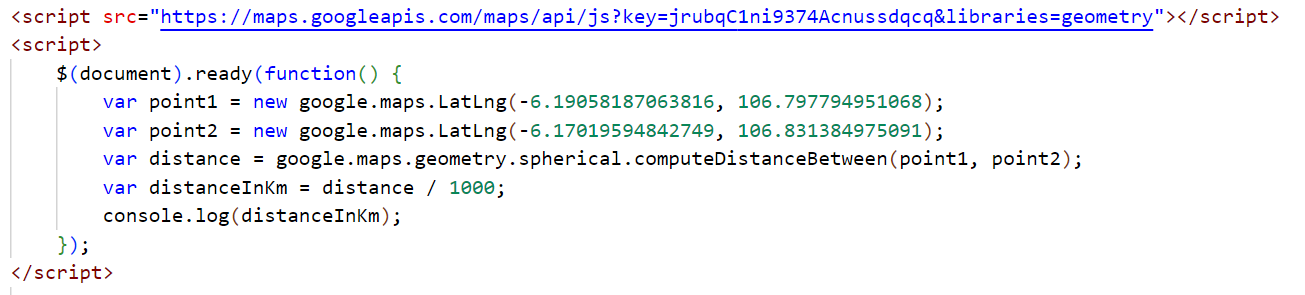
\includegraphics[width=13cm]{Gambar/bab3/google-geometry-library-api.png}
    	\caption{Kode Perhitungan Jarak \textit{Google Geometry Library} API}
    	\label{fig:kode-google-geometry-library-api}
    \end{figure}
    \FloatBarrier
%
\begin{longtable}{ |p{1cm}|p{3cm}|p{3cm}|p{3cm}|}
\caption{Tabel Perbandingan Algoritma Haversine Dengan \textit{Google Geometry Library} API}\label{tab:table-perbandingan-haversine-dan-google} 
\\
\hline
\textbf{No}
&\textbf{Lokasi}
&\textbf{Haversine Aplikasi Presensi (km)}
&\textbf{\textit{Google Geometry Library} (km)}
\\ 
\hline

\multirow{1}{*}{1}
&Universitas Tarumanagara
&2,5722
&2,5751
\\
\hline

\multirow{1}{*}{2}
&Gelora Bung Karno Stadium
&3,1518
&3,1554
\\
\hline

\multirow{1}{*}{3}
&Pasar Pecinan Glodok
&5,1614
&5,6212
\\
\hline

\multirow{1}{*}{4}
&Plaza Slipi Jaya
&0,2037
&0,2039
\\
\hline

\multirow{1}{*}{5}
&Pusat Jantung Nasional Harapan Kita
&0,5641
&0,5648
\\
\hline

\multirow{1}{*}{6}
&PIK Avenue
&11,0976
&11,1101
\\
\hline

\multirow{1}{*}{7}
&Thamrin City
&2,0578
&2,0602
\\
\hline

\multirow{1}{*}{8}
&Emporium Pluit
&7,0793
&7,0872
\\
\hline

\multirow{1}{*}{9}
&Apartemen Menteng Park
&4,6889
&4,6942
\\
\hline

\multirow{1}{*}{10}
&Central Park Mall
&1,5186
&1,5203
\\
\hline

\multirow{1}{*}{11}
&Summarecon Mall Serpong
&19,4990
&19,5208
\\
\hline

\multirow{1}{*}{12}
&Vihara Mahavira Graha Pusat
&7,3706
&7,3788
\\
\hline

\multirow{1}{*}{13}
&Stadium Patriot Candrabhaga
&22,1059
&22,1307
\\
\hline

\multirow{1}{*}{14}
&Pondok Zidane
&27,1100
&27,1404
\\
\hline

\multirow{1}{*}{15}
&Universitas Indonesia
&19,1874
&19.2089
\\
\hline

\multirow{1}{*}{16}
&Grand Galaxy Park
&21,2442
&21,2680
\\
\hline

\multirow{1}{*}{17}
&Museum Pancasila Sakti
&16,4728
&16,4913
\\
\hline

\multirow{1}{*}{18}
&Aeon Mall BSD City
&21,3194
&21,3433
\\
\hline

\multirow{1}{*}{19}
&Sarinah
&2,8680
&2,8712
\\
\hline

\multirow{1}{*}{20}
&Masjid Istiqlal
&4,3505
&4,3554
\\
\hline

\multirow{1}{*}{}
&\textbf{Rata-Rata}
&\textbf{10,0038}
&\textbf{10,0151}
\\
\hline

\end{longtable}

Hasil perhitungan rata-rata dari 20 koordinat lokasi yang dibandingkan dengan koordinat kantor MyPassword menggunakan Algoritma Haversine pada aplikasi presensi menunjukkan hasil 10,0038. Namun, ketika dibandingkan dengan hasil perhitungan menggunakan \textit{Google Geometry Library}, yang memiliki rata-rata 10,0151, terdapat perbedaan sebesar 0,0113. Hal ini menunjukkan adanya sedikit perbedaan antara hasil perhitungan Algoritma Haversine pada aplikasi dan \textit{Google Geometry Library}, namun selisih tersebut masih dalam batas toleransi yang dapat diterima untuk sebagian besar aplikasi praktis, termasuk aplikasi presensi.

\subsection{Pengujian Perhitungan Lembur}
Pada pengujian perhitungan lembur akan dilakukan beberapa skenario \textit{test case} untuk memastikan bahwa fitur perhitungan lembur dapat membuat dan menghitung data lembur secara otomatis jika \textit{Staff Infrastructure} melakukan presensi diluar penjadwalan \textit{shift} atau pada hari libur perusahaan. Sebelum melakukan pengujian akan terdapat beberapa konfigurasi yang dilakukan. Mengatur jenis shift yang terdiri dari hari Senin hingga Jumat mulai pukul 8 pagi hingga 5 sore dan hari Sabtu mulai pukul 8 pagi hingga 12 siang. \textbf{\ref{fig:pengaturan-jenis-shift}} menunjukkan hasil pengaturan hari pada jenis \textit{shift}.
\begin{figure}[!htbp]
    	\centering
    	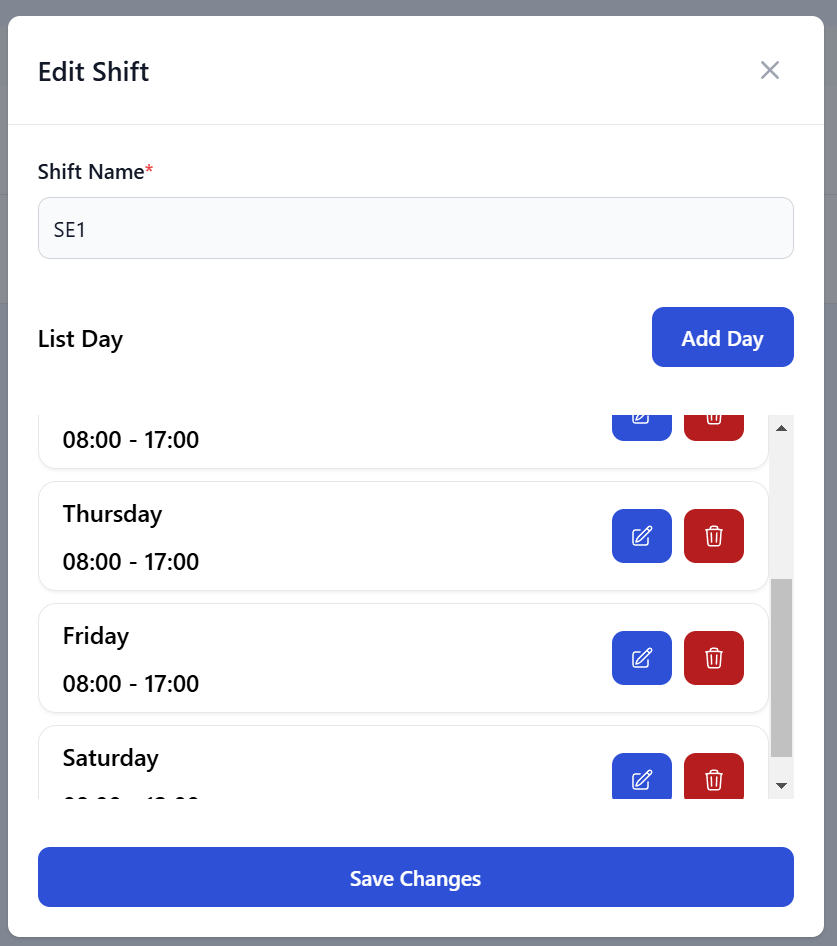
\includegraphics[width=9cm]{Gambar/bab4/pengaturan-jenis-shift.png}
    	\caption{Pengaturan Jenis \textit{Shift}}
    	\label{fig:pengaturan-jenis-shift}
        \end{figure}
        \FloatBarrier

Selanjutnya, menjadwalkan penggunaan jenis \textit{shift} yang telah dibuat sebelumnya dengan akun yang akan digunakan untuk pengujian. Jenis \textit{shift} akan dijadwalkan mulai tanggal 1 Januari 2024 hingga 31 Desember 2024. Hasil pengaturan penjadwalan \textit{shift} dapat dilihat pada \textbf{\ref{fig:pengaturan-penjadwalan-shift}}.
\begin{figure}[!htbp]
    	\centering
    	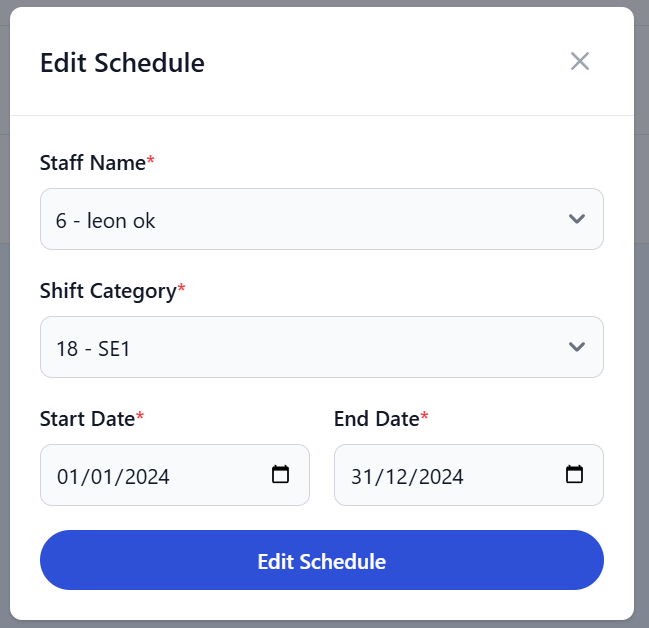
\includegraphics[width=9cm]{Gambar/bab4/pengaturan-penjadwalan-shift.png}
    	\caption{Pengaturan Penjadwalan \textit{Shift}}
    	\label{fig:pengaturan-penjadwalan-shift}
        \end{figure}
        \FloatBarrier

Setelah itu, membuat jenis libur baru yang berisi hari libur nasional Indonesia tahun 2024, penulis juga menambah libur pada tanggal 14 Desember 2024 sebagai pengujian. Hasil pembuatan jenis libur dapat dilihat pada \textbf{\ref{fig:pengujian-pengaturan-jenis-libur}}.
\begin{figure}[!htbp]
    	\centering
    	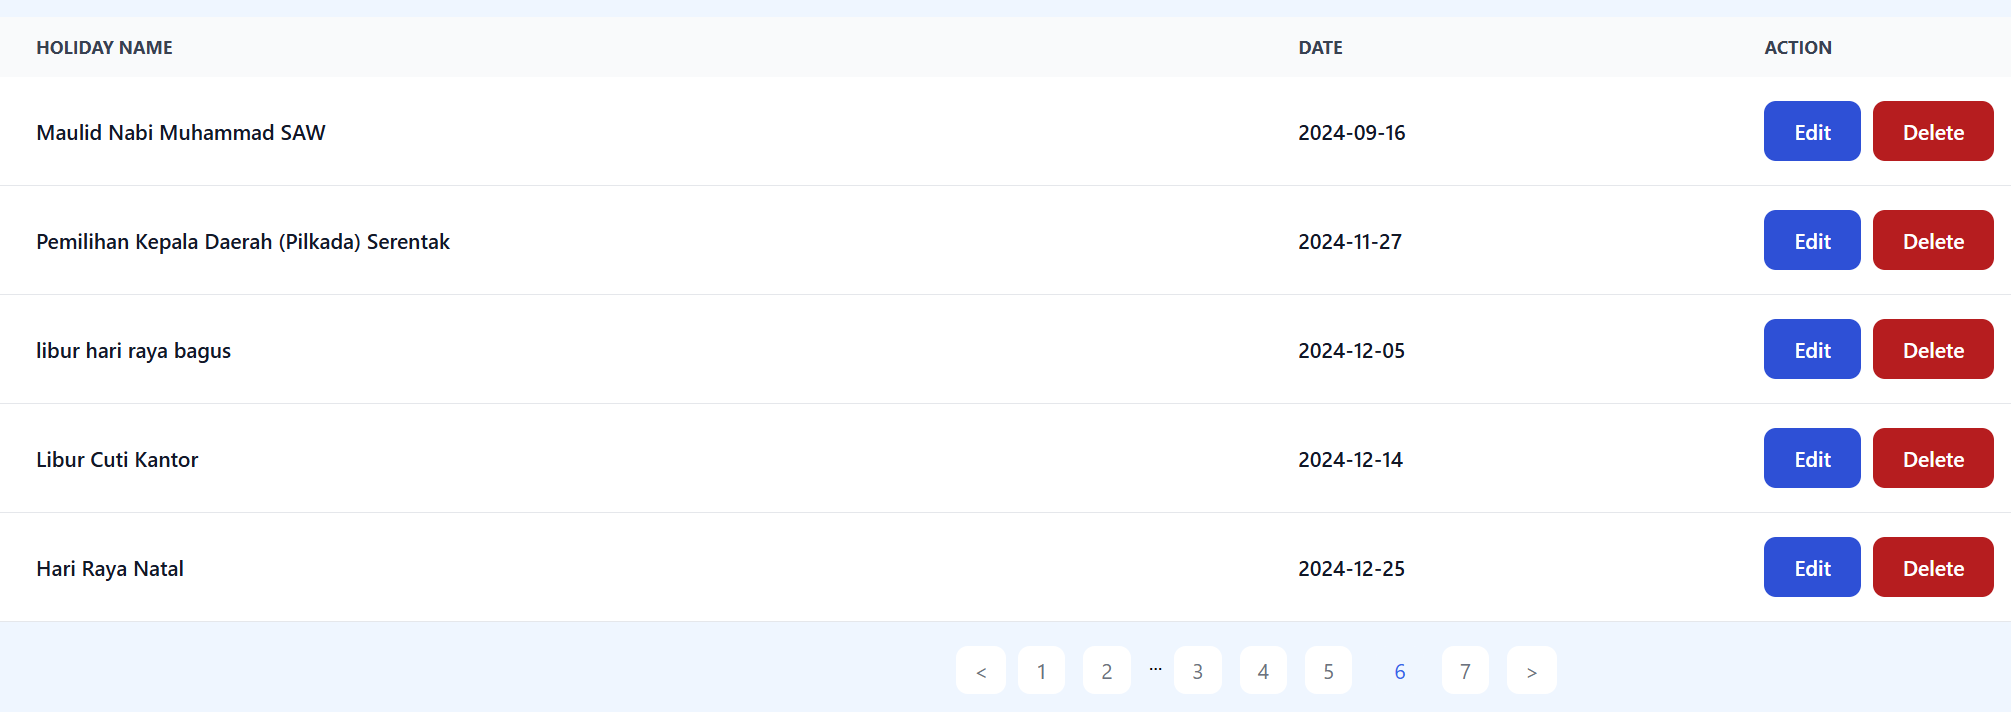
\includegraphics[width=17cm]{Gambar/bab4/pengaturan-jenis-libur.png}
    	\caption{Pengaturan Jenis Libur}
    	\label{fig:pengujian-pengaturan-jenis-libur}
        \end{figure}
        \FloatBarrier

Selanjtunya, menghubungkan akun yang akan digunakan sebagai pengujian dengan jenis libur yang telah dibuat sebelumnya melalui pengaturan \textit{user}. \textbf{\ref{fig:pengaturan-akun-user-dengan-jenis-libur}} menunjukkan hasil dari menghubungkan akun yang akan digunakan sebagai pengujian dengan jenis libur yang telah dibuat sebelumnya.
\begin{figure}[!htbp]
    	\centering
    	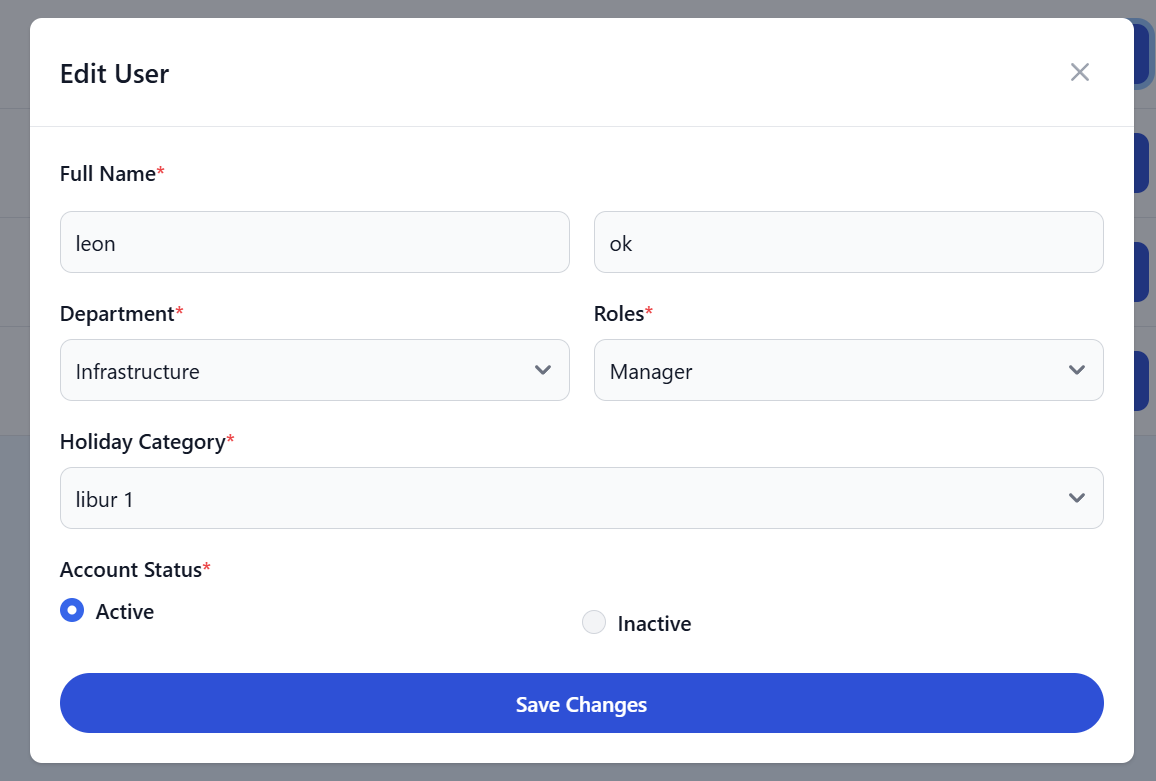
\includegraphics[width=9cm]{Gambar/bab4/pengaturan-pengaturan-user-libur.png}
    	\caption{Pengaturan Akun \textit{User} dengan Jenis Libur}
    	\label{fig:pengaturan-akun-user-dengan-jenis-libur}
        \end{figure}
        \FloatBarrier

Setelah \textit{shift} dan libur sudah dikonfigurasi, penulis melakukan pengujian pada skenario pertama yaitu melakukan presensi masuk pada hari Senin tanggal 12 Desember 2024 pukul 07.00 dan melakukan presensi keluar pada hari yang sama pukul 22.32. \textbf{\ref{fig:hasil-riwayat-presensi-skenario-pertama}} menunjukkan hasil riwayat presensi pada skenario pertama.
\begin{figure}[!htbp]
    	\centering
    	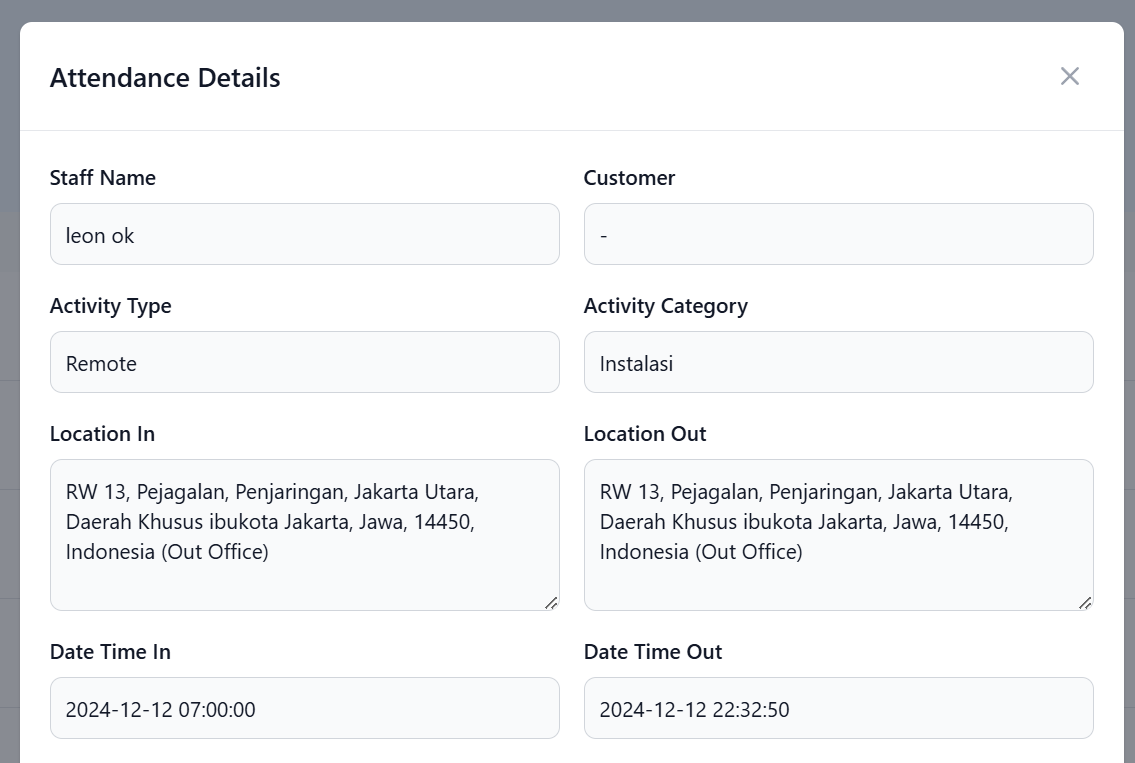
\includegraphics[width=9cm]{Gambar/bab4/pengujian-lembur-otomatis-attendance-1.png}
    	\caption{Hasil Riwayat Presensi Skenario Pertama}
    	\label{fig:hasil-riwayat-presensi-skenario-pertama}
        \end{figure}
        \FloatBarrier

Pada skenario pertama, sistem berhasil mendeteksi adanya lembur karena presensi masuk dilakukan sebelum \textit{shift} masuk dan presensi keluar dilakukan setelah \textit{shift} selesai. Sistem juga otomatis menghitung total jam lembur yaitu 6 jam 32 menit. Hasil riwayat lembur skenario pertama dapat dilihat pada \textbf{\ref{fig:hasil-riwayat-lembur-skenario-pertama}}.
\begin{figure}[!htbp]
    	\centering
    	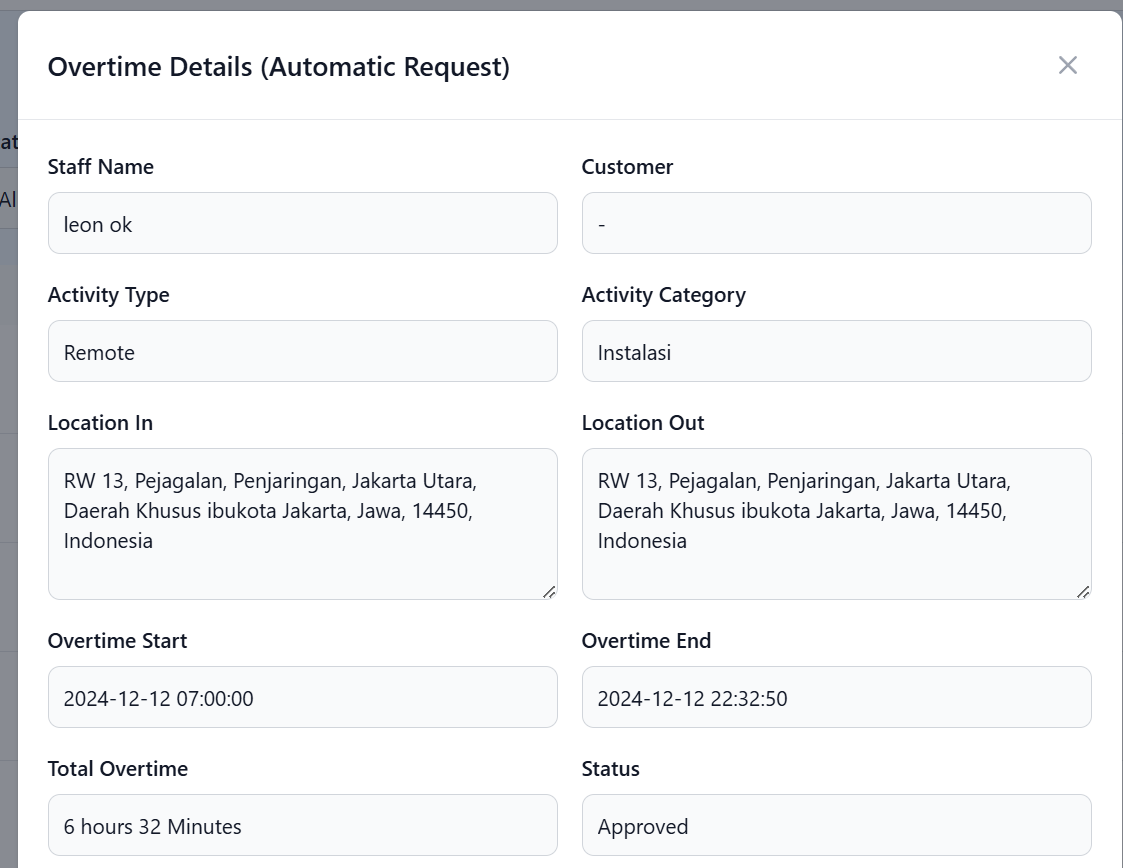
\includegraphics[width=9cm]{Gambar/bab4/pengujian-lembur-otomatis-overtime-1.png}
    	\caption{Hasil Riwayat Lembur Skenario Pertama}
    	\label{fig:hasil-riwayat-lembur-skenario-pertama}
        \end{figure}
        \FloatBarrier

Selanjutnya, pengujian skenario kedua dilakukan dengan melakukan presensi pada hari Senin tanggal 12 Desember 2024 pukul 17.30 dan presensi keluar pada hari yang sama pada pukul 22.27. Hasil riwayat presensi pada skenario kedua dapat dilihat pada \textbf{\ref{fig:hasil-riwayat-presensi-skenario-kedua}}.
\begin{figure}[!htbp]
    	\centering
    	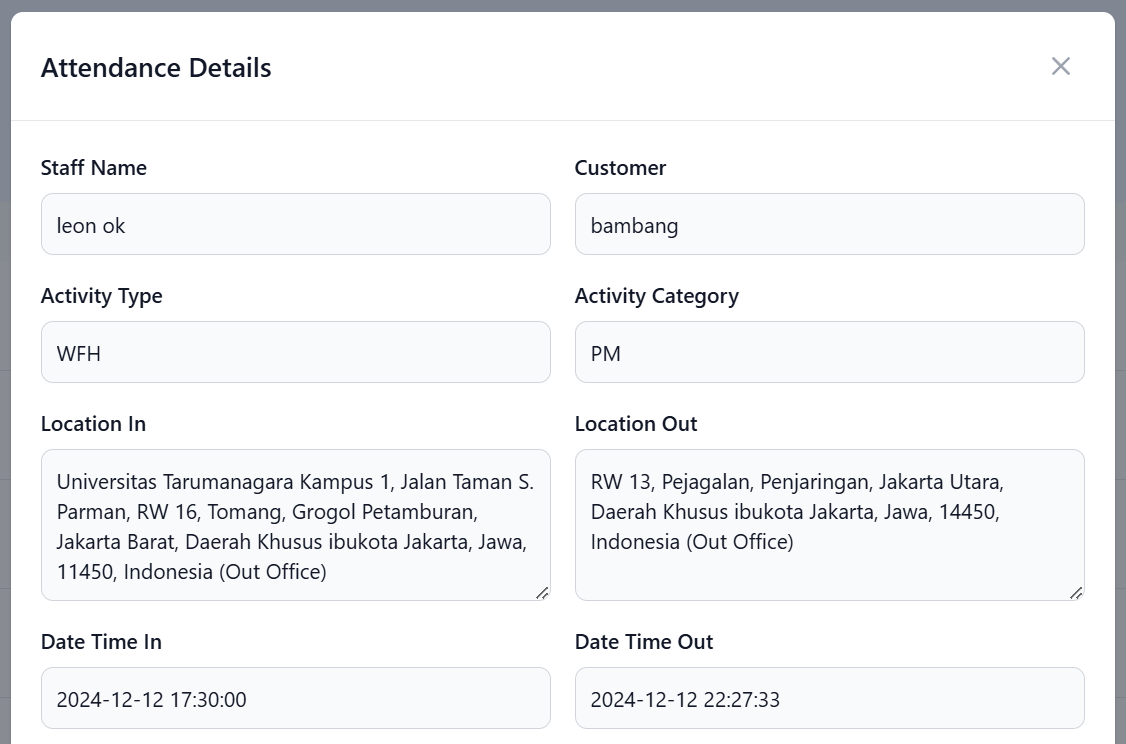
\includegraphics[width=9cm]{Gambar/bab4/pengujian-lembur-otomatis-attendance-2.png}
    	\caption{Hasil Riwayat Presensi Skenario Kedua}
    	\label{fig:hasil-riwayat-presensi-skenario-kedua}
        \end{figure}
        \FloatBarrier

Pada pengujian skenario kedua mendapatkan hasil yang sesuai. Sistem berhasil mendeteksi adanya lembur karena presensi masuk dan keluar dilakukan setelah \textit{shift} selesai. Sistem juga menghitung total jam lembur dengan hasil yang sesuai yaitu 4 jam 57 menit. Hasil riwayat lembur skenario kedua dapat dilihat pada \textbf{\ref{fig:hasil-riwayat-lembur-skenario-kedua}}.
\begin{figure}[!htbp]
    	\centering
    	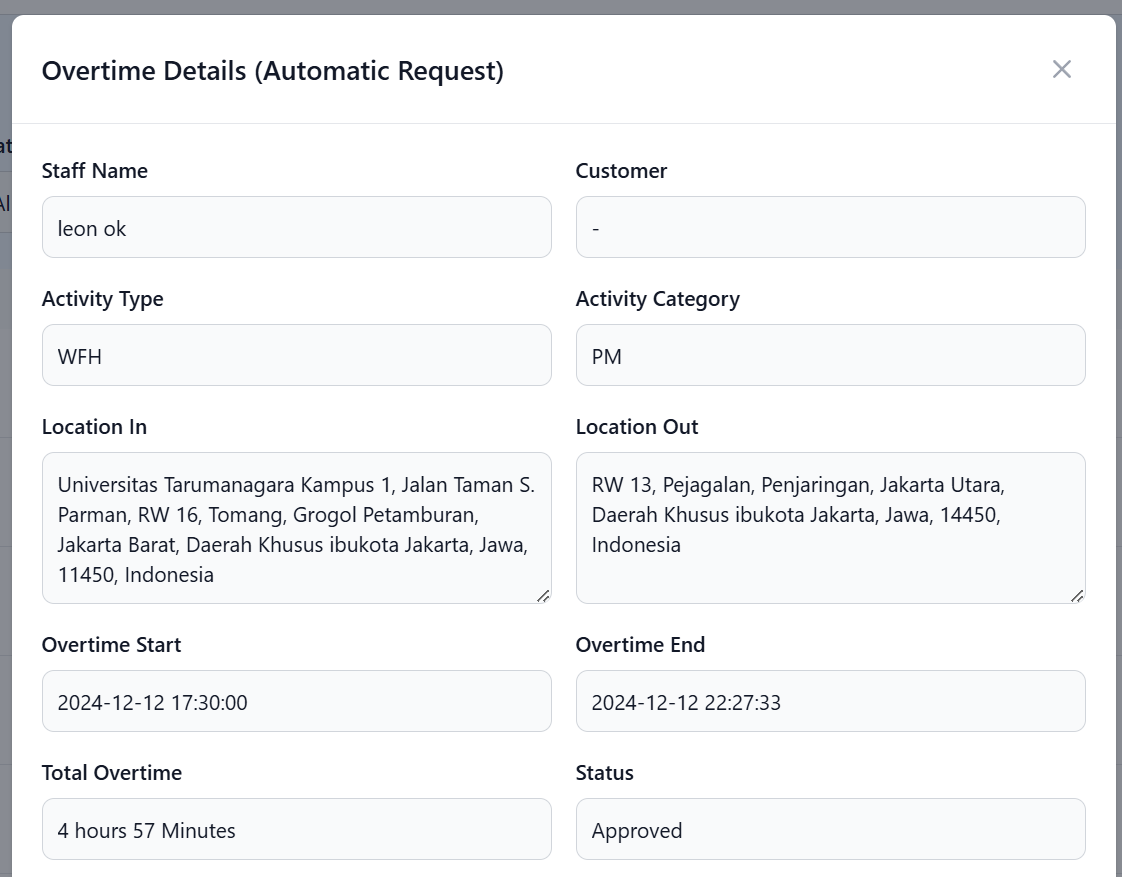
\includegraphics[width=9cm]{Gambar/bab4/pengujian-lembur-otomatis-overtime-2.png}
    	\caption{Hasil Riwayat Lembur Skenario Kedua}
    	\label{fig:hasil-riwayat-lembur-skenario-kedua}
        \end{figure}
        \FloatBarrier

Selanjutnya, pengujian pada skenario ketiga dilakukan dengan melakukan presensi masuk pada hari Senin tanggal 12 Desember 2024 pukul 22.33 dan presensi keluar pada hari yang berbeda yaitu Selasa tanggal 13 Desember 2024 pukul 09.46. Hasil riwayat presensi pada skenario ketiga dapat dilihat pada \textbf{\ref{fig:hasil-riwayat-presensi-skenario-ketiga}}.
\begin{figure}[!htbp]
    	\centering
    	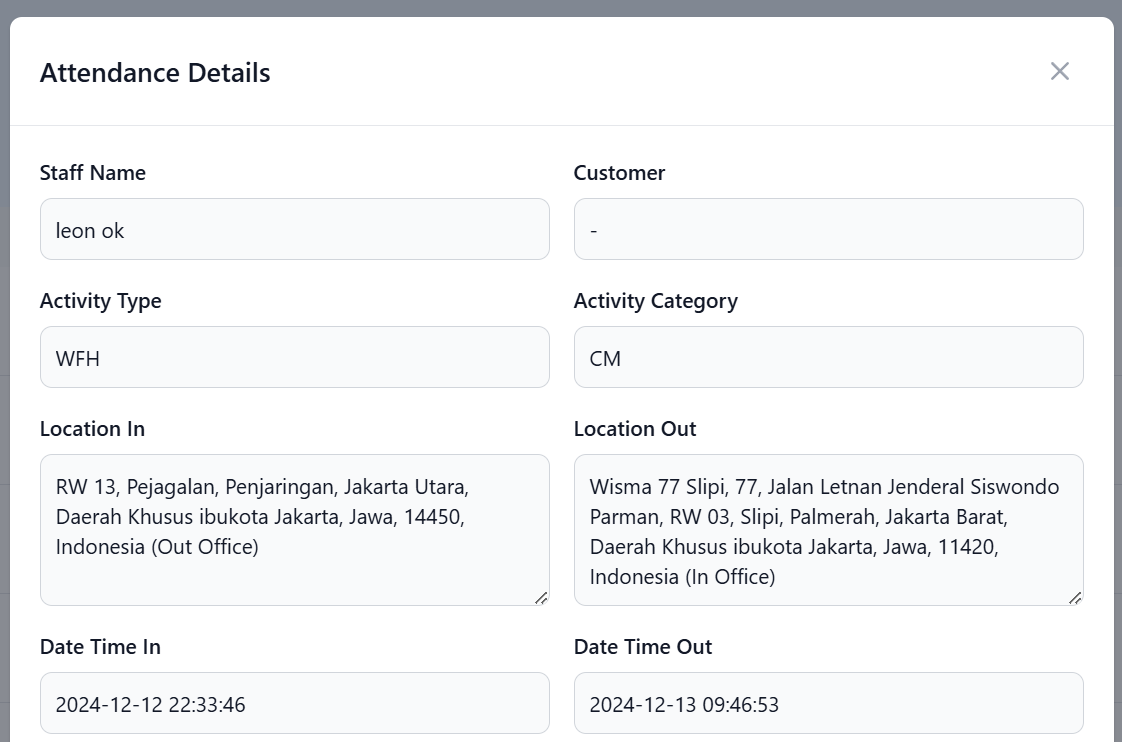
\includegraphics[width=9cm]{Gambar/bab4/pengujian-lembur-otomatis-attendance-3.png}
    	\caption{Hasil Riwayat Presensi Skenario Ketiga}
    	\label{fig:hasil-riwayat-presensi-skenario-ketiga}
        \end{figure}
        \FloatBarrier

Pada pengujian skenario ketiga, sistem berhasil mendeteksi adanya lembur karena presensi masuk dan keluar dilakukan setelah \textit{shift} selesai. Perhitungan total lembur juga sesuai walaupun presensi keluar dilakukan pada hari yang berbeda yaitu 9 jam 26 menit. Hasil riwayat lembur skenario ketiga dapat dilihat pada \textbf{\ref{fig:hasil-riwayat-lembur-skenario-ketiga}}.
\begin{figure}[!htbp]
    	\centering
    	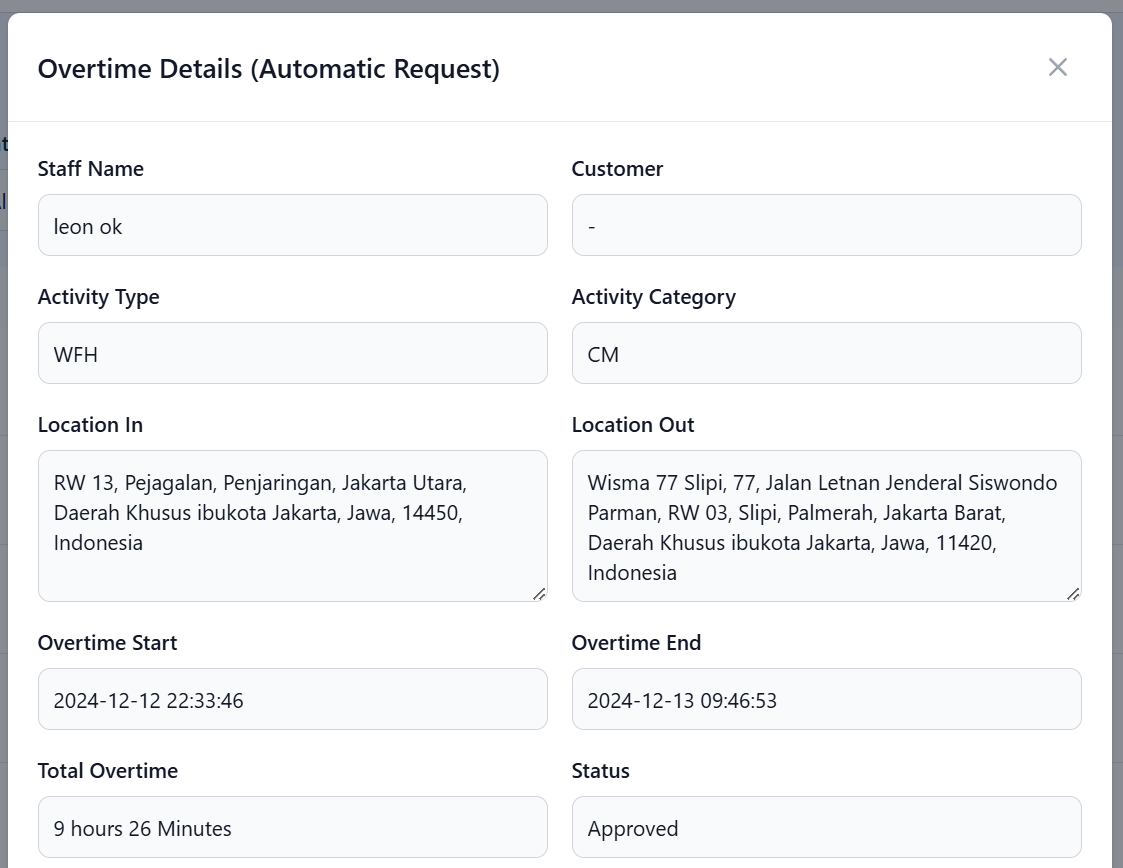
\includegraphics[width=9cm]{Gambar/bab4/pengujian-lembur-otomatis-overtime-3.png}
    	\caption{Hasil Riwayat Lembur Skenario Ketiga}
    	\label{fig:hasil-riwayat-lembur-skenario-ketiga}
        \end{figure}
        \FloatBarrier

Selanjutnya, pengujian pada skenario keempat dilakukan dengan melakukan presensi pada hari Selasa tanggal 13 Desember 2024 pukul 06.30 dan presensi keluar pada hari yang sama pukul 11.26. Hasil riwayat presensi pada skenario keempat dapat dilihat pada \textbf{\ref{fig:hasil-riwayat-presensi-skenario-keempat}}.
\begin{figure}[!htbp]
    	\centering
    	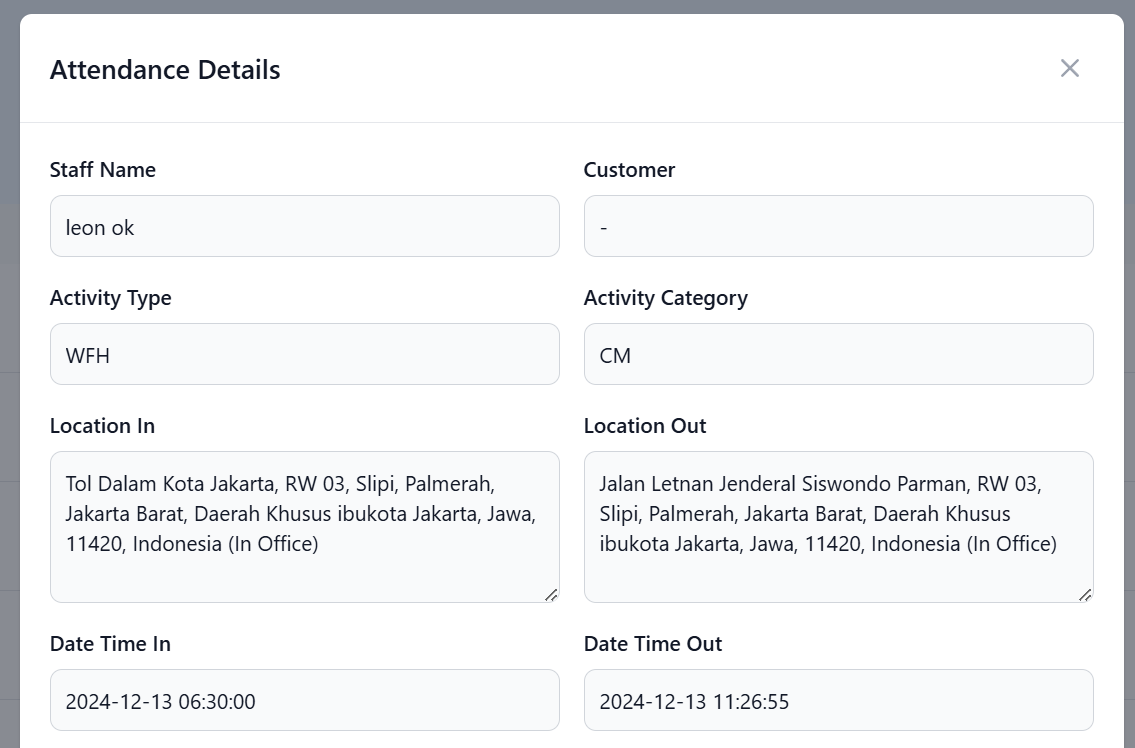
\includegraphics[width=9cm]{Gambar/bab4/pengujian-lembur-otomatis-attendance-4.png}
    	\caption{Hasil Riwayat Presensi Skenario Keempat}
    	\label{fig:hasil-riwayat-presensi-skenario-keempat}
        \end{figure}
        \FloatBarrier

Pada pengujian skenario keempat, sistem berhasil mendeteksi adanya lembur karena presensi masuk dilakukan sebelum \textit{shift} mulai. Sistem juga menghitung total lembur dengan hasil yang sesuai yaitu 1 jam 30 menit. Hasil riwayat lembur skenario keempat dapat dilihat pada \textbf{\ref{fig:hasil-riwayat-lembur-skenario-keempat}}.
\begin{figure}[!htbp]
    	\centering
    	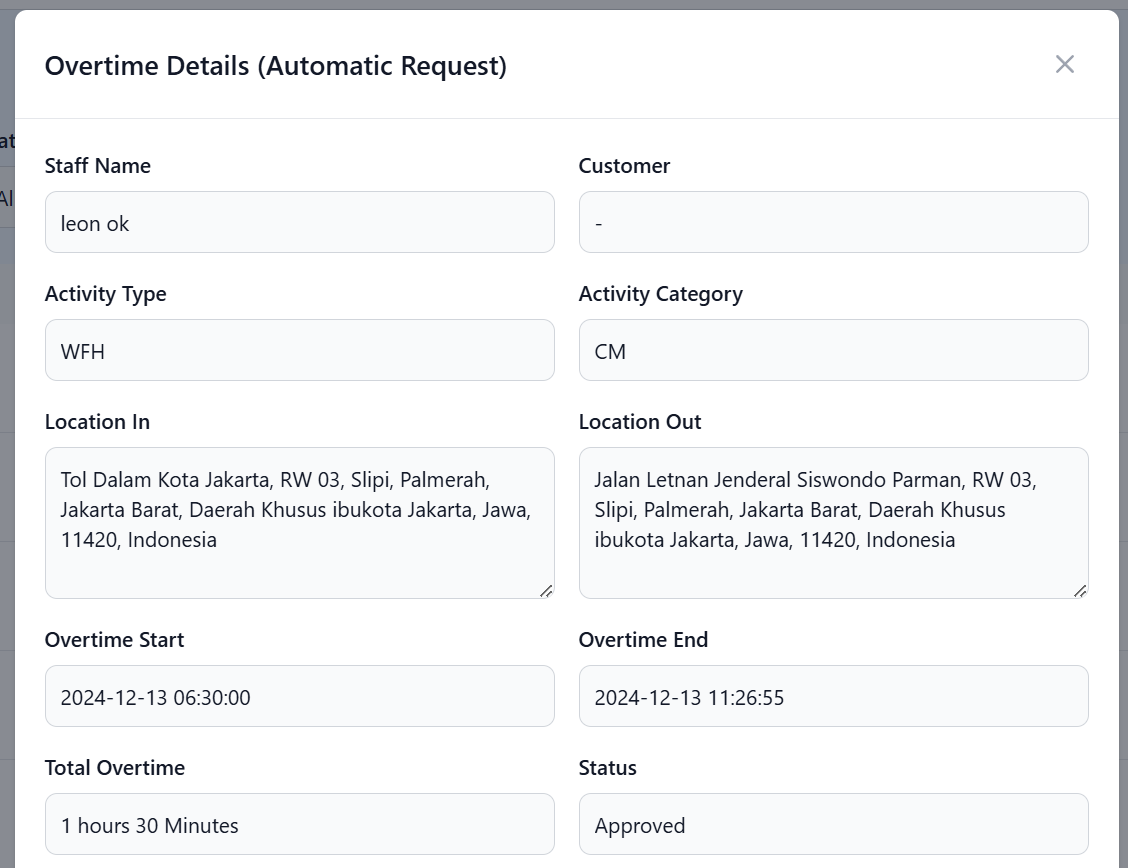
\includegraphics[width=9cm]{Gambar/bab4/pengujian-lembur-otomatis-overtime-4.png}
    	\caption{Hasil Riwayat Lembur Skenario Keempat}
    	\label{fig:hasil-riwayat-lembur-skenario-keempat}
        \end{figure}
        \FloatBarrier

Terakhir, skenario kelima akan dilakukan presensi masuk dan keluar saat \textit{shift}, namun pada hari tersebut terdapat hari libur perusahaan. Presensi masuk akan dilakukan pada hari Sabtu tanggal 14 Desember 2024 pukul 08.00 dan presensi keluar pada hari yang sama pukul 11.47. Hasil riwayat presensi pada skenario kelimat dapat dilihat pada \textbf{\ref{fig:hasil-riwayat-presensi-skenario-kelima}}.
\begin{figure}[!htbp]
    	\centering
    	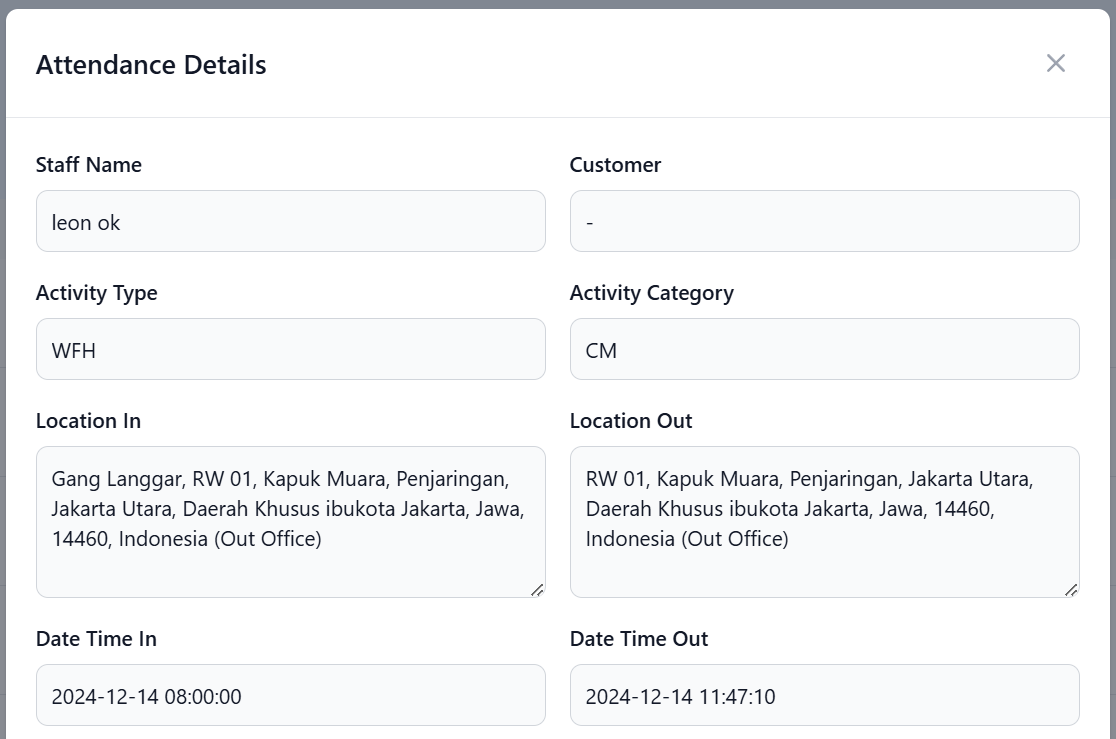
\includegraphics[width=9cm]{Gambar/bab4/pengujian-lembur-otomatis-attendance-5.png}
    	\caption{Hasil Riwayat Presensi Skenario Kelima}
    	\label{fig:hasil-riwayat-presensi-skenario-kelima}
        \end{figure}
        \FloatBarrier

Pada pengujian skenario kelima, sistem berhasil mendeteksi lembur walaupun pada hari tersebut terdapat \textit{shift} karena pada tanggal tersebut terdapat hari libur dari perusahaan. Sistem juga berhasil menghitung total jam lembur dengan sesuai yaitu 3 jam 47 menit. Hasil riwayat lembur skenario kelima dapat dilihat pada \textbf{\ref{fig:hasil-riwayat-lembur-skenario-kelima}}.
\begin{figure}[!htbp]
    	\centering
    	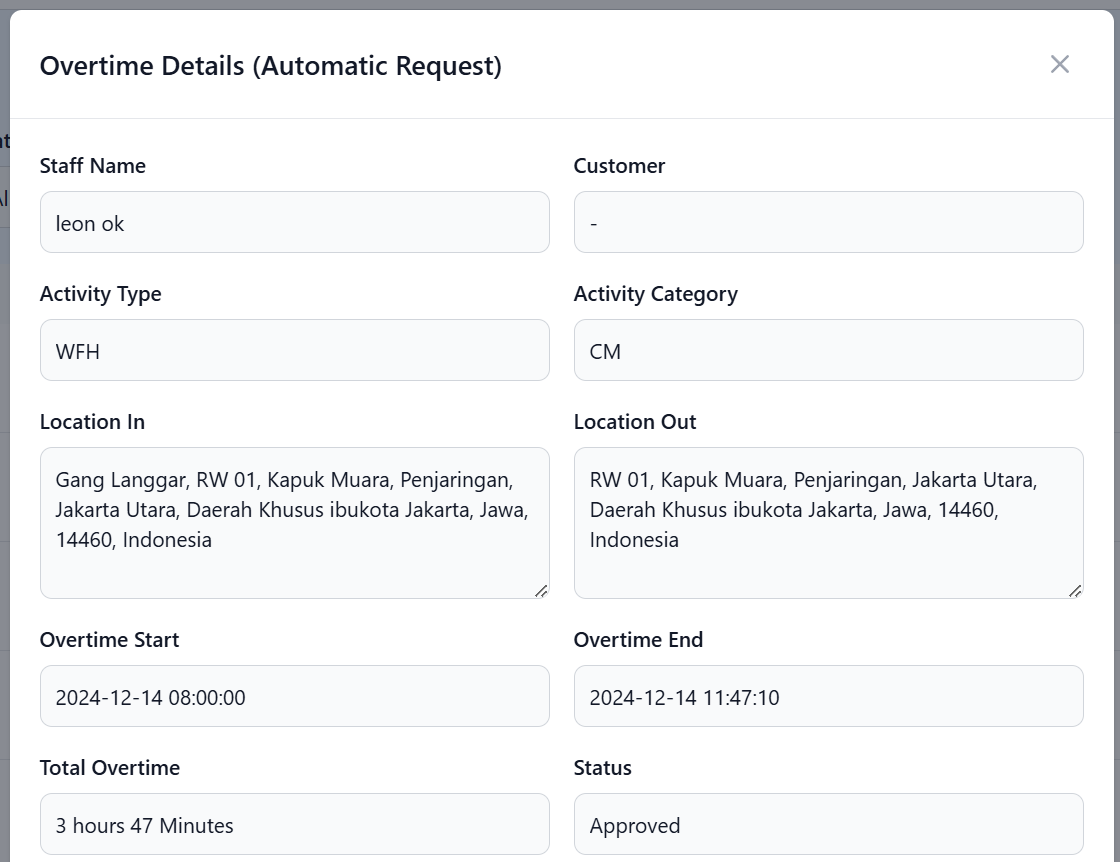
\includegraphics[width=9cm]{Gambar/bab4/pengujian-lembur-otomatis-overtime-5.png}
    	\caption{Hasil Riwayat Lembur Skenario Kelima}
    	\label{fig:hasil-riwayat-lembur-skenario-kelima}
        \end{figure}
        \FloatBarrier

Berdasarkan pengujian lembur otomatis dari 5 skenario yang berbeda, sistem berhasil mendeteksi adanya lembur jika presensi dilakukan diluar \textit{shift} yang telah ditentukan ataupun saat tanggal libur perusahaan. Sistem juga berhasil menghitung total jam lembur yang telah dilakukan dengan hasil yang akurat dan sesuai.

% \textbf{\ref{tab:table-skenario-perhitungan-lembur}} menunjukkan tabel hasil pengujian perhitungan lembur, seluruh tabel pengujian menunjukkan bahwa hasil yang diharapkan sesuai dengan hasil uji, sehingga dapat disimpulkan bahwa pengujian berhasil memenuhi semua kriteria yang telah ditetapkan.

% \begin{longtable}{ |p{1cm}|p{1.5cm}|p{1.5cm}|p{1.5cm}|p{3cm}|p{3cm}|}
% \caption{Tabel Skenario \textit{Test Case} Perhitungan Lembur}\label{tab:table-skenario-perhitungan-lembur} 
% \\
% \hline
% \textbf{Libur}
% &\textbf{Jadwal \textit{Shift}}
% &\textbf{Presensi Masuk}
% &\textbf{Presensi Keluar}
% &\textbf{Hasil Uji}
% &\textbf{Hasil Yang Diharapkan}
% \\ 
% \hline

% \multirow{1}{*}{Tidak}
% &Senin 08:00-17:00
% &Senin 06:00
% &Senin 08:00
% &Data lembur akan tercatat dengan total waktu 120 menit.
% &Data lembur berhasil tercatat dengan total waktu 120 menit.
% \\
% \hline

% \multirow{1}{*}{Tidak}
% &Senin 08:00-17:00
% &Senin 07:00
% &Senin 19:00
% &Data lembur akan tercatat dengan total waktu 180 menit.
% &Data lembur berhasil tercatat dengan total waktu 180 menit.
% \\
% \hline

% \multirow{1}{*}{Tidak}
% &Senin 08:00-17:00
% &Senin 17:00
% &Senin 18:15
% &Data lembur akan tercatat dengan total waktu 75 menit.
% &Data lembur berhasil tercatat dengan total waktu 75 menit.
% \\
% \hline

% \multirow{1}{*}{Tidak}
% &Senin 08:00-17:00
% &Senin 23:00
% &Selasa 01:00
% &Data lembur akan tercatat dengan total waktu 120 menit.
% &Data lembur berhasil tercatat dengan total waktu 120 menit.
% \\
% \hline

% \multirow{1}{*}{Ya}
% &Senin 08:00-17:00
% &Senin 08:00
% &Senin 12:00
% &Data lembur akan tercatat dengan total waktu 240 menit.
% &Data lembur berhasil tercatat dengan total waktu 240 menit.
% \\
% \hline


% \end{longtable}

\subsection{Pengujian TensorFlow}
Pada pengujian TensorFlow akan dilakukan dengan percobaaan pengambilan foto wajah melalui kamera perangkat pada saat presensi. Pada pengujian ini akan dilakukan beberapa skenario \textit{test case}. Pada skenaro pertama, akan dilakukan pengambilan foto saat presensi dengan tidak ada wajah pada kamera yang dapat dilihat pada \textbf{\ref{fig:pengambilan-foto-tidak-ada-wajah}}. Hasil yang diharapkan dari skenario ini adalah menampilkan pesan \textit{error} bahwa tidak ada wajah pada kamera. Hasil pengujian dapat dilihat pada \textbf{\ref{fig:hasil-uji-tidak-ada-wajah}}. Berdasarkan hasil pengujian dari skenario pertama didapatkan hasil yang sesuai dengan yang diharapkan.

Selanjutnya pada skenario kedua, akan dilakukan pengambilan foto wajah dengan posisi kepala diluar lingkaran putih pada kamera. \textbf{\ref{fig:pengambilan-foto-tidak-ditengah}} menunjukkan pengambilan foto wajah dengan posisi kepala diluar lingkaran putih. Hasil yang diharapkan dari skenario tersebut adalah menampilkan pesan \textit{error} bahwa pengambilan wajah, posisi kepala harus berada didalam lingkaran putih yang dapat dilihat pada \textbf{\ref{fig:hasil-uji-wajah-tidak-ditengah}}. Berdasarkan hasil pengujian didapatkan hasil yang sesuai dengan yang diharapkan.

\begin{figure}[!htbp]
    	\centering
    	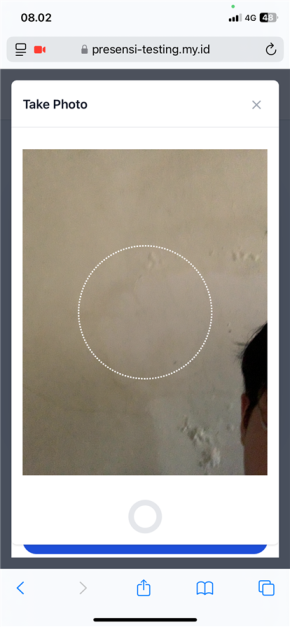
\includegraphics[width=4cm]{Gambar/bab4/pengambilan-foto-tidak-ada-wajah.PNG}
    	\caption{Tidak Ada Wajah Saat Pengambilan Foto}
    	\label{fig:pengambilan-foto-tidak-ada-wajah}
        \end{figure}
        \FloatBarrier

        \begin{figure}[!htbp]
    	\centering
    	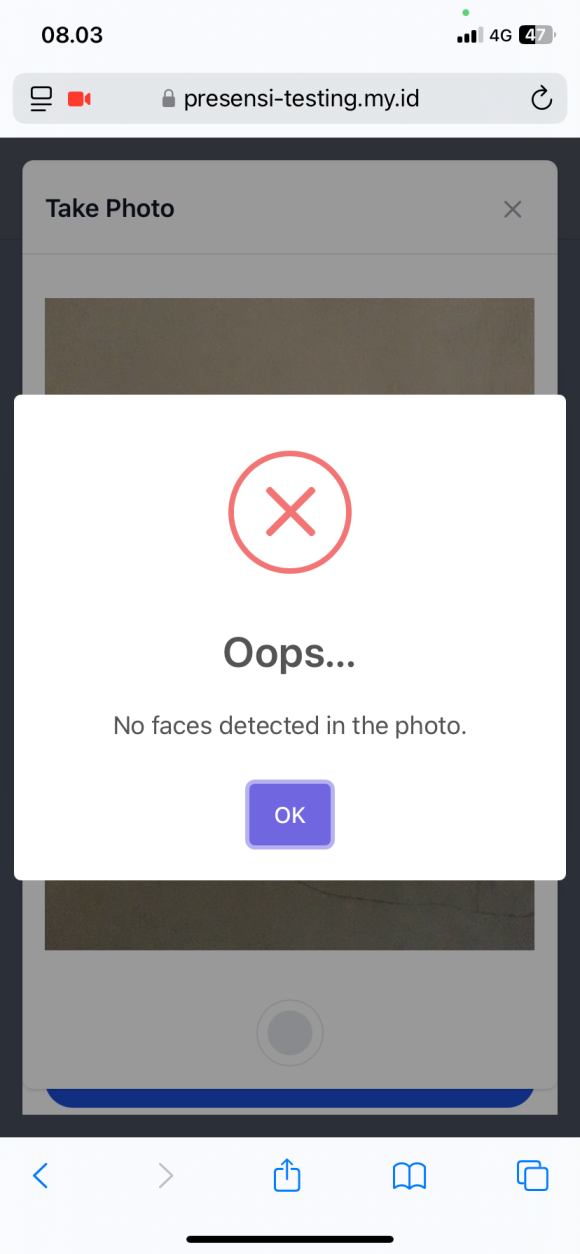
\includegraphics[width=4cm]{Gambar/bab4/hasil-uji-tidak-ada-wajah.PNG}
    	\caption{Hasil Uji Tidak Ada Wajah Saat Pengambilan Foto}
    	\label{fig:hasil-uji-tidak-ada-wajah}
        \end{figure}
        \FloatBarrier

\begin{figure}[!htbp]
    	\centering
    	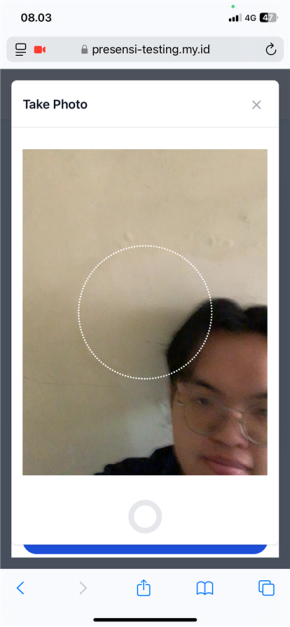
\includegraphics[width=4cm]{Gambar/bab4/pengambilan-foto-tidak-ditengah.PNG}
    	\caption{Posisi Wajah Tidak Ditengah Saat Pengambilan Foto}
    	\label{fig:pengambilan-foto-tidak-ditengah}
        \end{figure}
        \FloatBarrier

        \begin{figure}[!htbp]
    	\centering
    	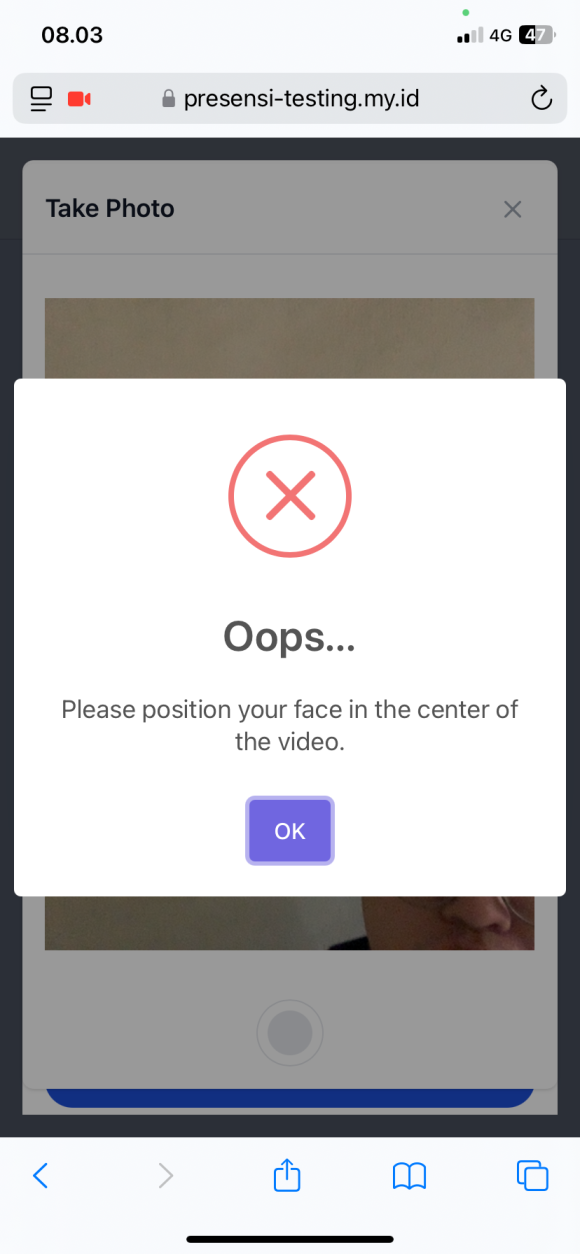
\includegraphics[width=4cm]{Gambar/bab4/hasil-uji-wajah-tidak-ditengah.PNG}
    	\caption{Hasil Uji Posisi Wajah Tidak Ditengah Saat Pengambilan Foto}
    	\label{fig:hasil-uji-wajah-tidak-ditengah}
        \end{figure}
        \FloatBarrier

Setelah itu, pada skenario ketiga dilakukan pengambilan foto wajah didalam lingkaran putih, namun posisi kepala terlalu dekat dengan kamera sehingga posisi kepala keluar dari batas lingkaran putih yang dapat dilihat pada \textbf{\ref{fig:pengambilan-foto-terlalu-dekat}}. Hasil yang diharapkan dari skenario ini yaitu menampilkan pesan \textit{error} bahwa wajah terlalu dekat dengan kamera. \textbf{\ref{fig:hasil-uji-wajah-terlalu-dekat}} menunjukkan hasil yang didapat dari pengujian. Berdasarkan hasil pengujian didapatkan hasil yang sesuai dengan yang diharapkan.

\begin{figure}[!htbp]
    	\centering
    	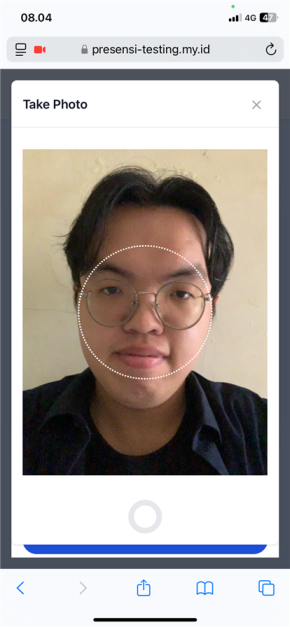
\includegraphics[width=4cm]{Gambar/bab4/pengambilan-foto-terlalu-dekat.PNG}
    	\caption{Posisi Wajah Dekat Dengan Kamera Saat Pengambilan Foto}
    	\label{fig:pengambilan-foto-terlalu-dekat}
        \end{figure}
        \FloatBarrier

        \begin{figure}[!htbp]
    	\centering
    	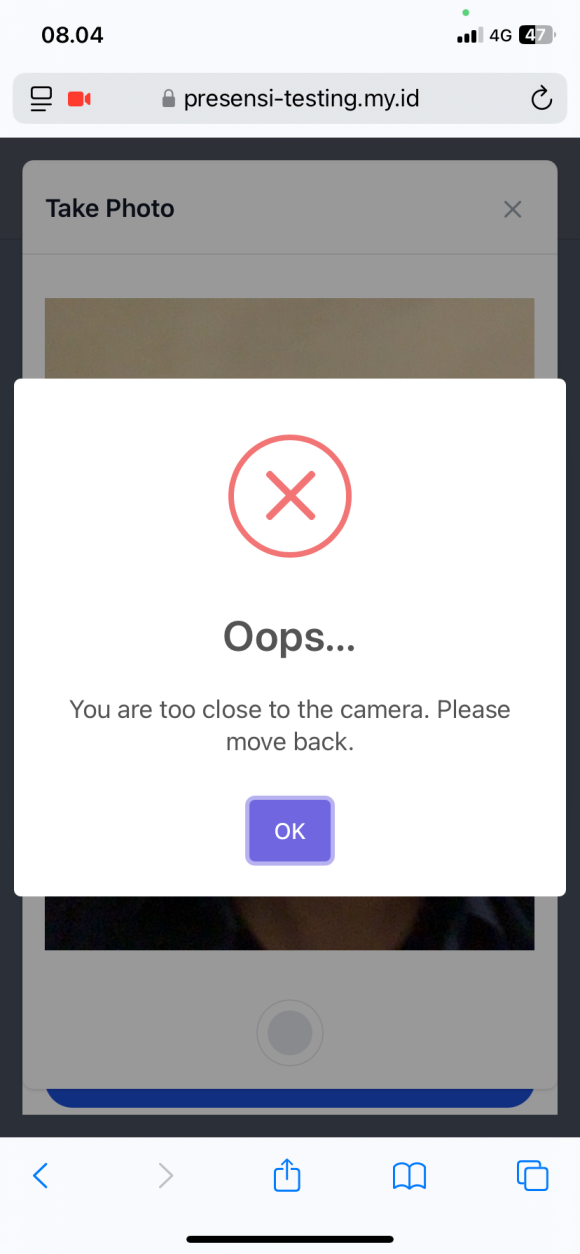
\includegraphics[width=4cm]{Gambar/bab4/hasil-uji-wajah-terlalu-dekat.PNG}
    	\caption{Hasil Uji Posisi Wajah Dekat Dengan Kamera Saat Pengambilan Foto}
    	\label{fig:hasil-uji-wajah-terlalu-dekat}
        \end{figure}
        \FloatBarrier

Terakhir, pada skenario keempat dilakukan pengambilan foto wajah yang tepat posisinya didalam lingkaran putih yang dapat dilihat pada \textbf{\ref{fig:pengambilan-foto-pas}}. Hasil yang diharapkan dari pengujian ini adalah modal Kamera akan tertutup dan menampilkan hasil \textit{preview} foto pada modal presensi. Hasil pengujian dapat dilihat pada \textbf{\ref{fig:hasil-uji-foto-pas}}. Berdasarkan hasil pengujian didapatkan hasil yang sesuai dengan yang diharapkan. Seluruh skenario pengujian memberikan hasil yang sesuai sehingga fitur validasi wajah pada aplikasi presensi \textit{online} berfungsi dengan baik.

\begin{figure}[!htbp]
    	\centering
    	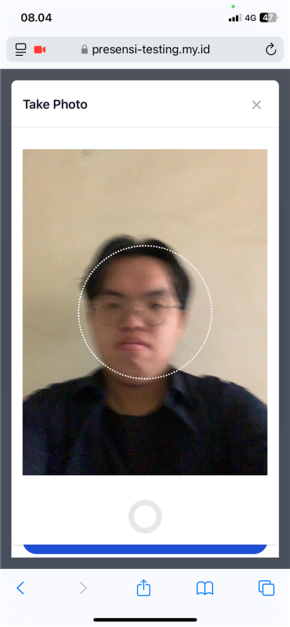
\includegraphics[width=4cm]{Gambar/bab4/pengambilan-foto-pas.PNG}
    	\caption{Posisi Wajah Tepat Didalam Lingkaran Saat Pengambilan Foto}
    	\label{fig:pengambilan-foto-pas}
        \end{figure}
        \FloatBarrier

        \begin{figure}[!htbp]
    	\centering
    	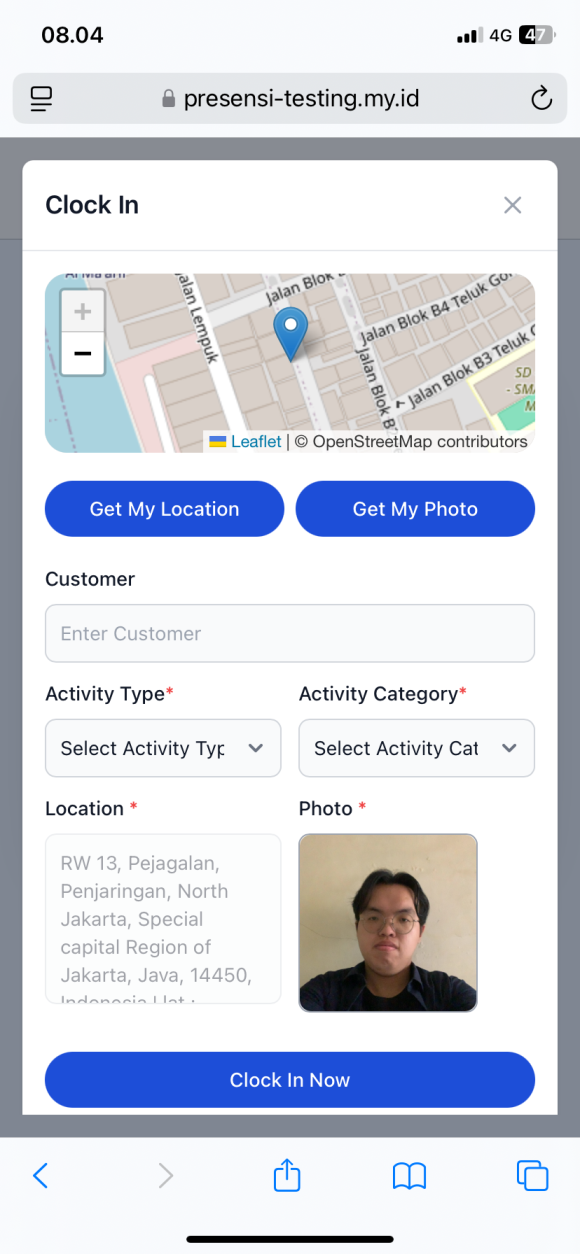
\includegraphics[width=4cm]{Gambar/bab4/hasil-uji-foto-pas.PNG}
    	\caption{Hasil Uji Posisi Wajah Tepat Didalam Lingkaran Saat Pengambilan Foto}
    	\label{fig:hasil-uji-foto-pas}
        \end{figure}
        \FloatBarrier

\subsection{Pengujian oleh Pengguna \textit{Non}-IT}
Pengujian oleh user \textit{non}-IT akan dilakukan menggunakan metode \textit{blackbox testing}, seperti yang telah dilakukan sebelumnya, serta metode SUS (\textit{System Usability Scale}) kepada \textit{staff} MyPassword yang bekerja di divisi \textit{non}-IT seperti \textit{sales, driver, product specialist, business support, digital marketing,} dan \textit{admin}. Pengujian dilakukan pada tanggal 12 hingga 13 Desember 2024 secara luring di MyPassword. Hasil pengujian \textit{blackbox testing} kepada \textit{staff} MyPassword divisi \textit{non-}IT dapat dilihat pada \textbf{\hyperref[sec:blackbox-testing-aplikasi-presensi-online-oleh-pengguna-non-it]{Lampiran~XIX}}.

Selanjutnya dilakukan juga SUS (\textit{System Usability Scale}) kepada \textit{staff} MyPassword divisi \textit{non-}IT. Menurut Albert dan Tullis~\cite{measuring2022bill}, SUS (\textit{System Usability Scale}) merupakan salah satu alat yang paling banyak digunakan untuk menilai persepsi kegunaan suatu sistem atau produk. SUS terdiri dari 10 pernyataan yang dinilai oleh pengguna berdasarkan tingkat kesetujuan pengguna. Setengah dari pernyataan tersebut menggunakan kata-kata positif, sementara setengah lainnya menggunakan kata-kata negatif. Skala kesetujuan 5 poin digunakan untuk setiap pernyataan yang terdiri dari pilihan sangat setuju, setuju, ragu-ragu, tidak setuju, dan sangat tidak setuju. Berikut ini adalah 10 pertanyaan pada pengujian SUS:
\begin{enumerate}
    \item Saya berpikir bahwa saya akan sering menggunakan sistem ini.
    \item Saya merasa sistem ini terlalu rumit tanpa alasan.
    \item Saya merasa sistem ini mudah digunakan.
    \item Saya berpikir bahwa saya akan membutuhkan bantuan teknisi untuk dapat menggunakan sistem ini.
    \item Saya merasa berbagai fungsi dalam sistem ini terintegrasi dengan baik.
    \item Saya merasa ada terlalu banyak inkonsistensi dalam sistem ini.
    \item Saya membayangkan bahwa kebanyakan orang akan cepat belajar menggunakan sistem ini.
    \item Saya merasa sistem ini sangat merepotkan untuk digunakan.
    \item Saya merasa sangat percaya diri menggunakan sistem ini.
    \item Saya perlu mempelajari banyak hal sebelum bisa mulai menggunakan sistem ini.
\end{enumerate}

Cara untuk menghitung skor SUS yaitu dengan menjumlahkan kontribusi skor dari setiap pertanyaan, di mana setiap kontribusi skor bernilai antara 0 hingga 4. Untuk pertanyaan bernomor ganjil (1, 3, 5, 7, dan 9), kontribusi skor dihitung dengan mengurangi 1 dari posisi pada skala. Sedangkan untuk pertanyaan bernomor genap (2, 4, 6, 8, dan 10), kontribusinya dihitung dengan mengurangi posisi pada skala dari 5. Setelah semua kontribusi dijumlahkan, kalikan hasilnya dengan 2,5 untuk memperoleh skor SUS secara keseluruhan. Hasil dari perhitungan skor SUS digunakan untuk menentukan peringkat. \textbf{\ref{fig:tabel-peringkat-sus}} menunjukkan peringkat berdasarkan skor SUS.
\begin{figure}[!htbp]
    	\centering
    	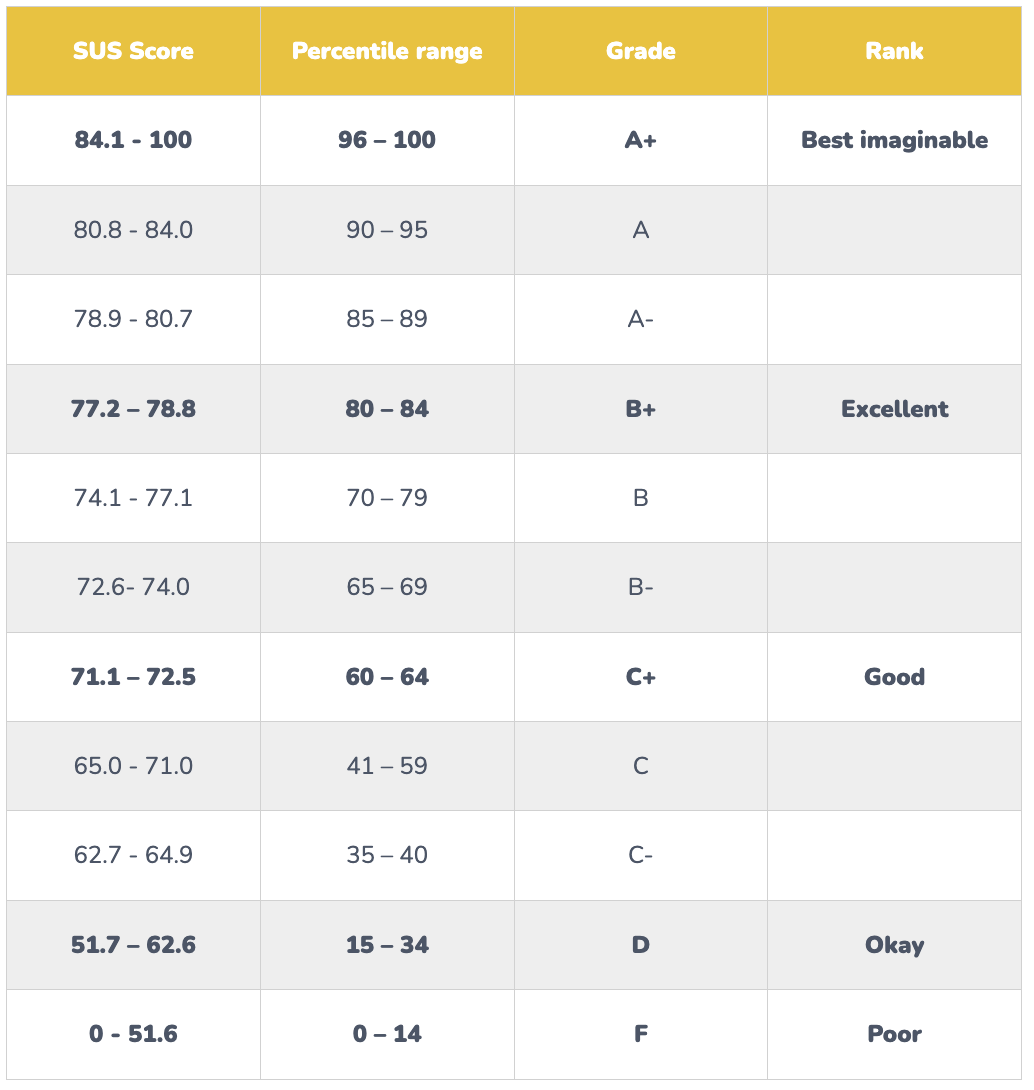
\includegraphics[width=10cm]{Gambar/bab4/tabel-peringkat-sus.png}
    	\caption{Peringkat SUS\cite{system2024john}}
    	\label{fig:tabel-peringkat-sus}
        \end{figure}
        \FloatBarrier

\begin{figure}[!htbp]
    	\centering
    	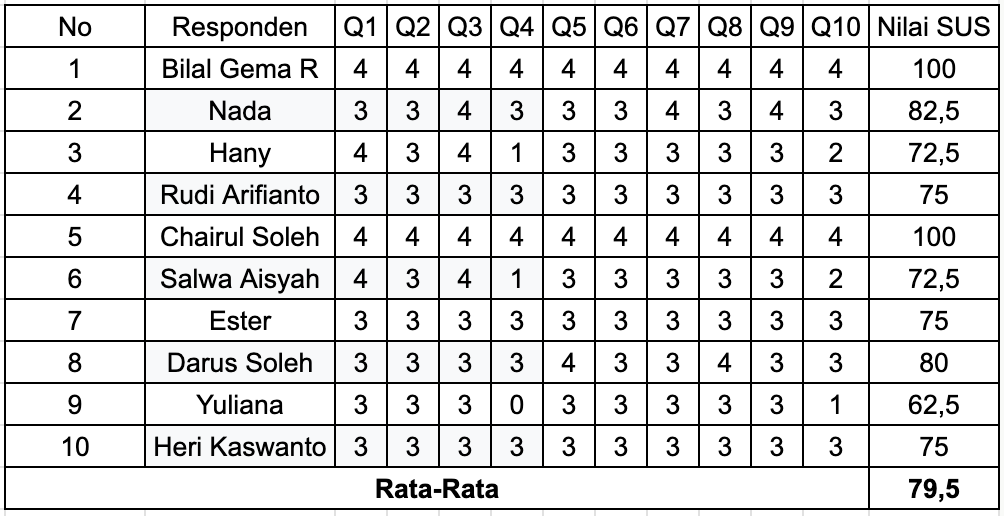
\includegraphics[width=13cm]{Gambar/bab4/hasil-sus.png}
    	\caption{Hasil Pengujian SUS}
    	\label{fig:hasil-pengujian-sus}
        \end{figure}
        \FloatBarrier
        
Pengujian SUS pada aplikasi presensi \textit{online} berbasis web menggunakan \textit{Google Form} melalui tautan \url{https://forms.gle/WrkckqFsDjx8AryZ6}. Pada pengujian ini didapatkan 10 responden yang memiliki rentang umur antara 24-53 tahun dengan latar belakang pekerjaan \textit{non}-IT. Hasil pengujian SUS dengan \textit{staff} MyPassword \textit{non-}IT dapat dilihat pada \textbf{\ref{fig:hasil-pengujian-sus}}. Grafik hasil pengujian dan perhitungan skor SUS dapat dilihat pada \textbf{\ref{fig:grafik-pengujian-sus}}. Berdasarkan rata-rata hasil pengujian SUS dari 10 responden, diperoleh skor SUS sebesar 79,5, yang termasuk dalam peringkat A- pada skala SUS.
\begin{figure}[!htbp]
    	\centering
    	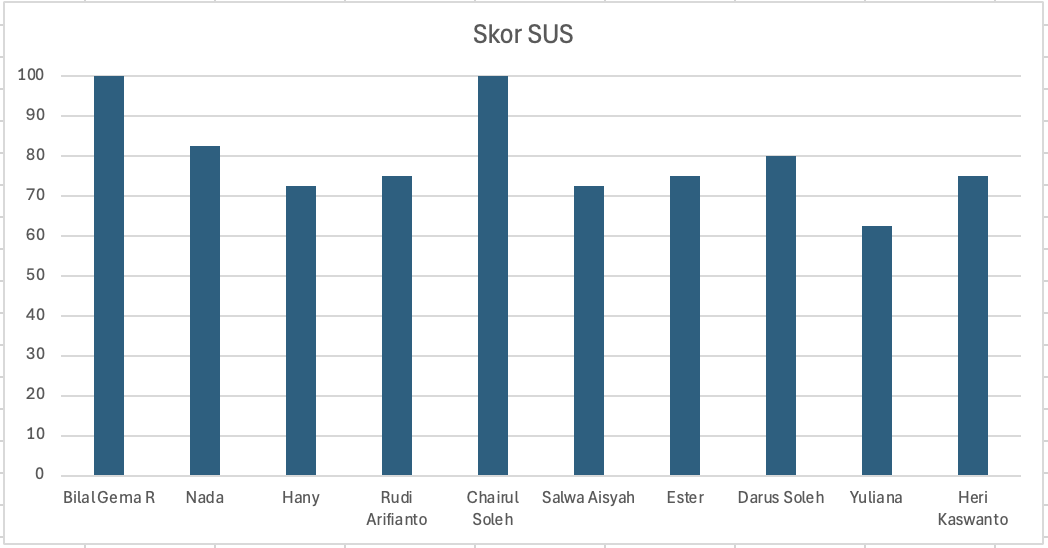
\includegraphics[width=13cm]{Gambar/bab4/grafik-sus.png}
    	\caption{Grafik Pengujian SUS}
    	\label{fig:grafik-pengujian-sus}
        \end{figure}
        \FloatBarrier

Dokumentasi pengujian \textit{blackbox testing} dan pengujian SUS bersama \textit{staff} MyPassword dengan latar belakang pekerjaan \textit{non-}IT dapat dilihat pada \textbf{\hyperref[sec:dokumentasi-blackbox-testing-dan-sus-bersama-staff-non-it]{Lampiran~XX}}.